\chapter{Automatisation du processus d'investigation}
\label{Automatisation du processus d'investigation}
\thispagestyle{fancy}


\section{Architecture High Level du système proposé}
\label{Automatisation du processus d'investigation: Achitecture High Level du système proposé}
En s'appuyant sur les définitions et l'architecture High Level du Machine Learning (partie \ref{Le Machine Learning: Généralités sur le Machine Learning: Définition et principe général}), on propose un schéma synoptique haut niveau de la solution proposée (figure, en réponse à la problématique. 

\begin{figure}[h]
	\centering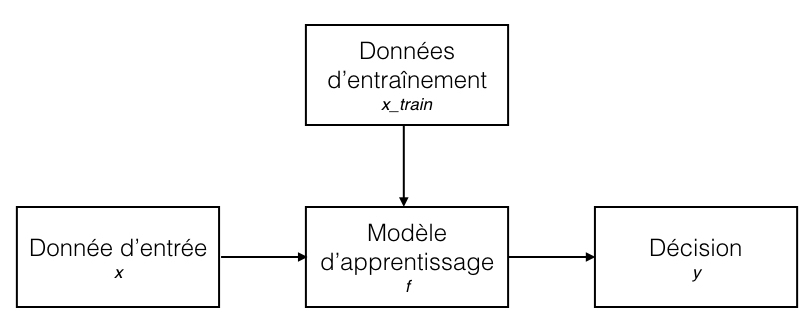
\includegraphics[height=5cm]{images/ML_high_level.jpeg}
	\caption{Schéma synoptique haut niveau de la solution proposée}
	\label{fig:Schéma synoptique haut niveau de la solution proposée}
\end{figure}

\section{Solutions techniques testées}
\label{Automatisation du processus d'investigation: Solutions techniques testées}




\section{Solution technique proposée}
\label{Automatisation du processus d'investigation: Solution technique proposée}

